There are two basic approaches to meshing a B-rep,
namely (1) to represent the geometry by means of `voxels'\cite{Bu07Trea},
or (2) to mesh the surface, then generate a volume mesh that coincides with
the surface mesh.

\begin{figure}
\centerline{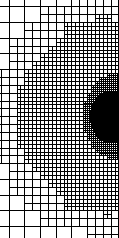
\includegraphics[width=8cm]{../png/amrmesh}}
\caption{An AMR mesh surrounding a curved body drawn as solid black at right.\label{fig:amr}}
\end{figure}
Voxels are the volume equivalent of pixels, so that the geometry
is represented by a uniform cuboid lattice of geometrically
identical cells, each possibly labelled with a set of physical properties.
Refinements of voxelisation are to allow
clusters of small cells to be treated as larger
cuboid bodies~\cite{Va05CTan}, and to omit cells altogether within say solid surfaces
(also known as `tartan meshing'). When both techniques are combined in say CFD,
the result is known as an AMR mesh, see \Fig{amr}.

\begin{figure}
\centerline{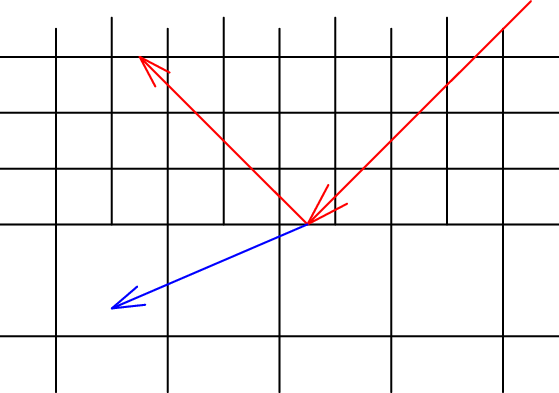
\includegraphics[width=8cm]{../png/iamr}}
\caption{Spurious reflections when using low order scheme with AMR\label{fig:amrefl}}
\end{figure}

As suggested by the previous paragraph, an AMR mesher is potentially quite complicated.
A well-known difficulty with schemes that use AMR meshes is illustrated by \Fig{amrefl}.
There will be interfaces between meshes of different size, even in regions with
the same physical properties. However, a wave with a wavelength of less than~$10h$, where
$h$ is the local mesh-spacing, modelled using a second-order accurate scheme,
has a propagation speed in error by~$1$\,\%, which
error increases as $h^p$~typically with $p=2$. Thus computationally, the
region show in \Fig{amrefl} may have different dispersion properties at
shorter wavelength in the two different grid-sizes, and computations will
exhibit a spurious reflection at the interface, which may be misleading or even
destabilising in certain cases.
The importance of the work of Nikiforakis et al~\cite{Go18Dime} is that they
have managed to produce in effect a spatio-temporal AMR mesh, so that they can
compute the equations of inviscid compressible FD \emph{explicitly} using a local timestep.
Such meshes have also been successfully used for Particle-in-Cell calculations of
extreme complexity for spacecraft charging~\cite{Mi16part}, meaning that Nikiforakis
work deserved attention. Unfortunately,
considerable discussion of the merits of the Nikiforakis approach versus spectral
element at the Birmingham meeting~\cite{y1re111b} indicated potentially severe difficulties for
AMR meshes when diffusion, especially anisotropic diffusion has to be treated.

\subsection{Importance of Geometrical Accuracy} \label{sec:codegeom}
The approximate nature of the intersection between two NURBS surfaces may also cause
difficulties, as indicated by \Fig{meshes}. Power deposition
on the PFCs shielding may depend critically on the direction of the surface normal.
A grid of planar triangles may produce errors like those indicated by
\Fig{meshes}(a), whereas more faithful representations would resemble
\Fig{meshes}(b).
\begin{figure}[h]
\centerline{(a){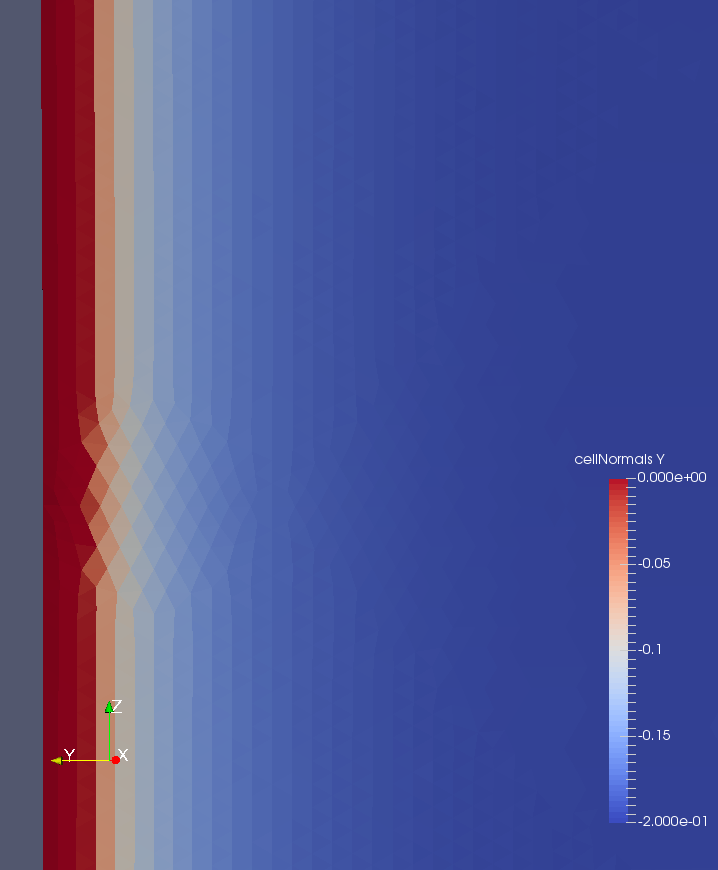
\includegraphics[width=7.0cm]{../png/meshbad.png}}
(b) {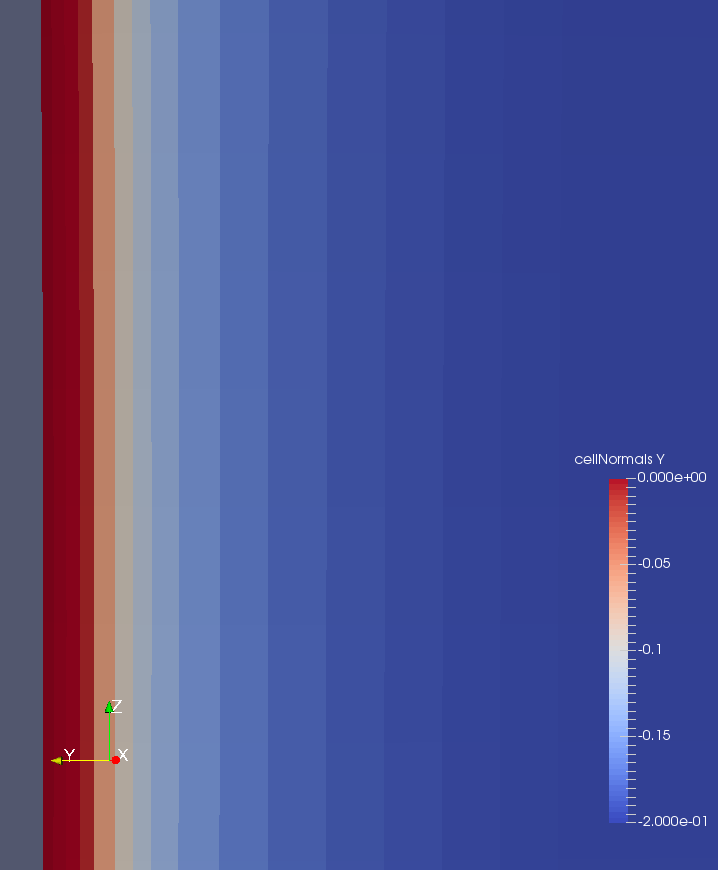
\includegraphics[width=7.0cm]{../png/meshgood.png}}
}
\caption{Close-ups of two triangular meshes of the central left edge surface
of a TBM Tungsten shield.  The  CAD contains a join in the middle of the image
leading to the irregular behaviour of the horizontal component of surface normal
in the image at left~(a). Refitting of CAD using the CADfix$^{TM}$ software package
enables the production of a more smoothly
varying normal, see mesh at right~(b).
\label{fig:meshes}}
\end{figure}



A difficulty for both AMR and surface-based approaches is the order of error~$p_s$ in the spatial approximation of
surfaces and other interfaces used to bound the domain of a PDE calculation.
The important result is by Boffi~\cite{Bo12Infl} that
the results of a PDE calculation can have order no higher than~$p_s$. Thus in the
usual approach that starts by meshing the surface with simple planar triangles, there is
no point in using schemes of high or spectral order. Many  meshing packages allow only for
second order surface approximations, whereby typically each side of say a `curved' triangle is 
represented by three points and hence a quadratic fit. Notable exceptions
are gmsh~\cite{Ge09gmsh} and MFEM~\cite{Do20hrad,mfemwebsite}.

\begin{figure}
\centerline{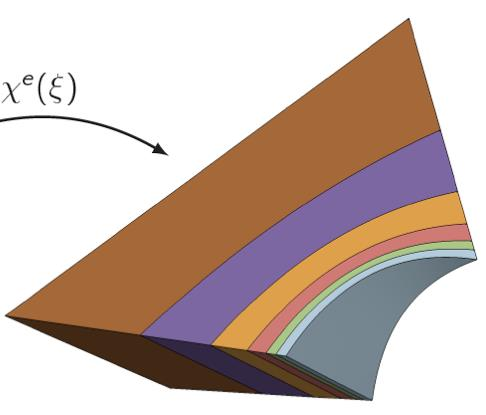
\includegraphics[width=8cm]{../png/shmo-754}}
\centerline{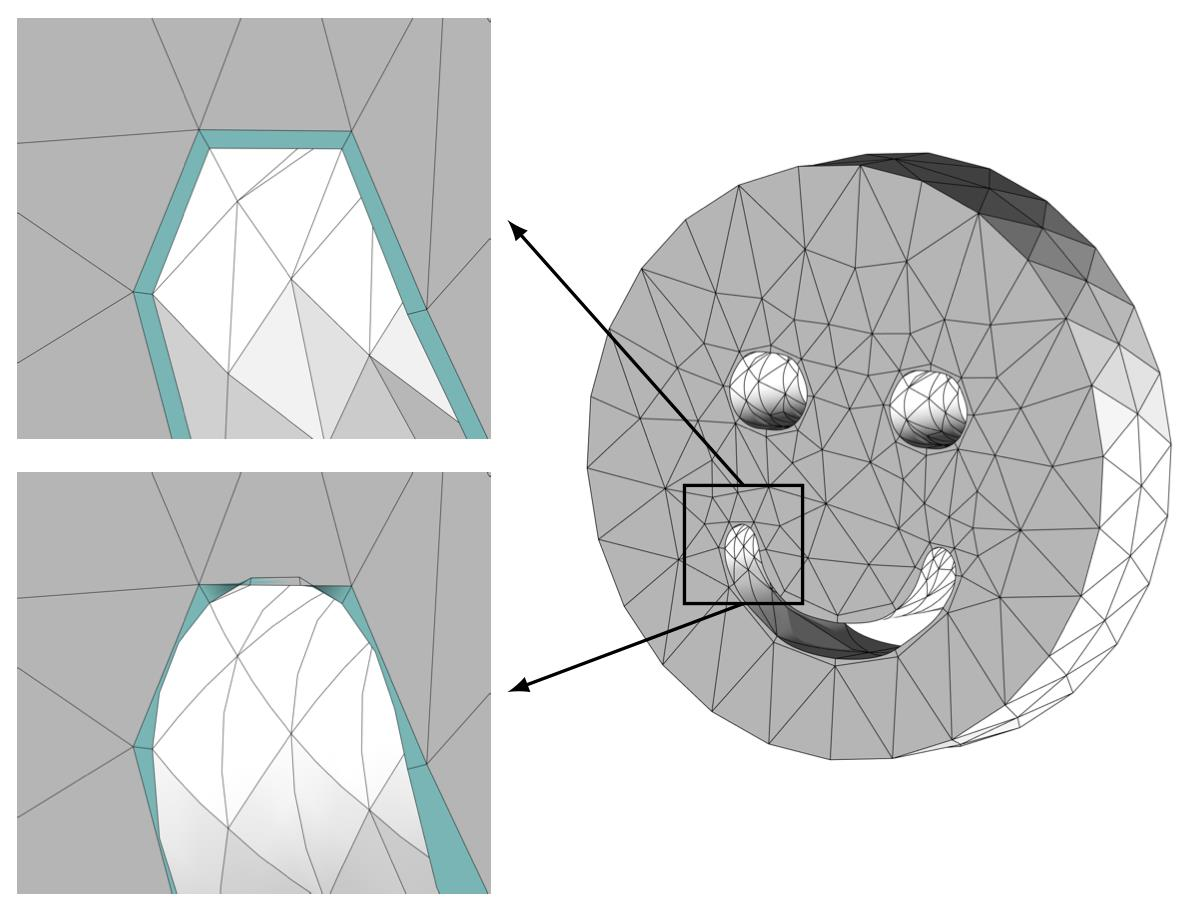
\includegraphics[width=8cm]{../png/shmo-672}}
\centerline{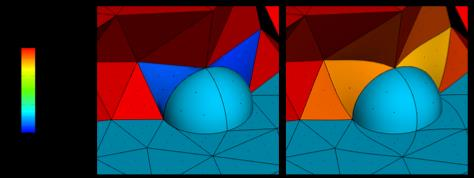
\includegraphics[width=8cm]{../png/shmo-681}}
\caption{At top is illustrated a desirable meshing close to a curved surface, when eg.\ small
scale physical effects due to a sheath need to be represented. Below is an indication
of how packages may fail when they try to produce this mesh using low-order spatially
spatially accurate elements (planar triangles), from a presentation by Sherwin and Moxey
at CCFE\label{fig:meshprob}
At bottom is a second picture from the same presentation, showing resolution
of a problem arising when mesh is tangent to a surface.}
\end{figure}

Consultations indicate difficulties with higher-order spatially accurate meshing
even for relatively simple geometries that might be encountered in the tokamak edge.
\Fig{meshprob} shows two problems. The first is where  self-intersection occurs when
trying to insert nodes  inside thin elements near curved boundaries. The other is
where the surface triangulation has a tangency to an extrusion. The Nekmesh
software is being developed~\cite{Tu17fram,Tu18Curv} using concepts from optimisation theory to 
treat such issues.

\clearpage
\subsection{Example Meshing Problem} \label{sec:meshprob}
A example text case is formed by the meshing of the surface JET Tile~1~(T1),
which is one of the vertical tiles at the left of the divertor in \Fig{jetdive}.
The figures containing surface meshes are taken from a study in ref~[RP4,\S\,5.1]\cite{Wa19}
that attempted to find a minimal, accurate mesh representation for the 
T1 surfaces receiving power.
\begin{figure}
\centerline{
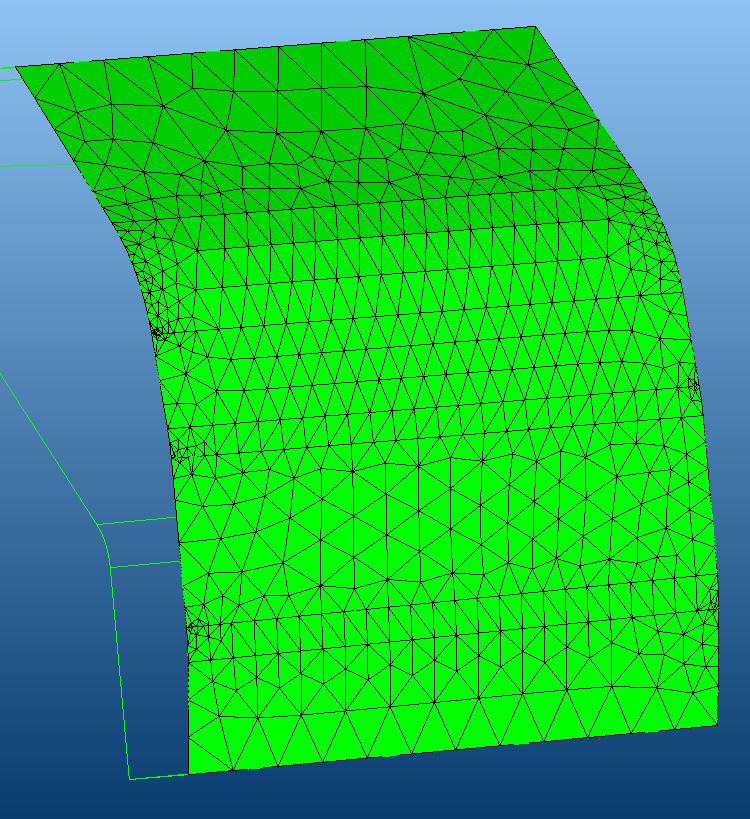
\includegraphics[width=0.42\columnwidth]{../png/t2t5}
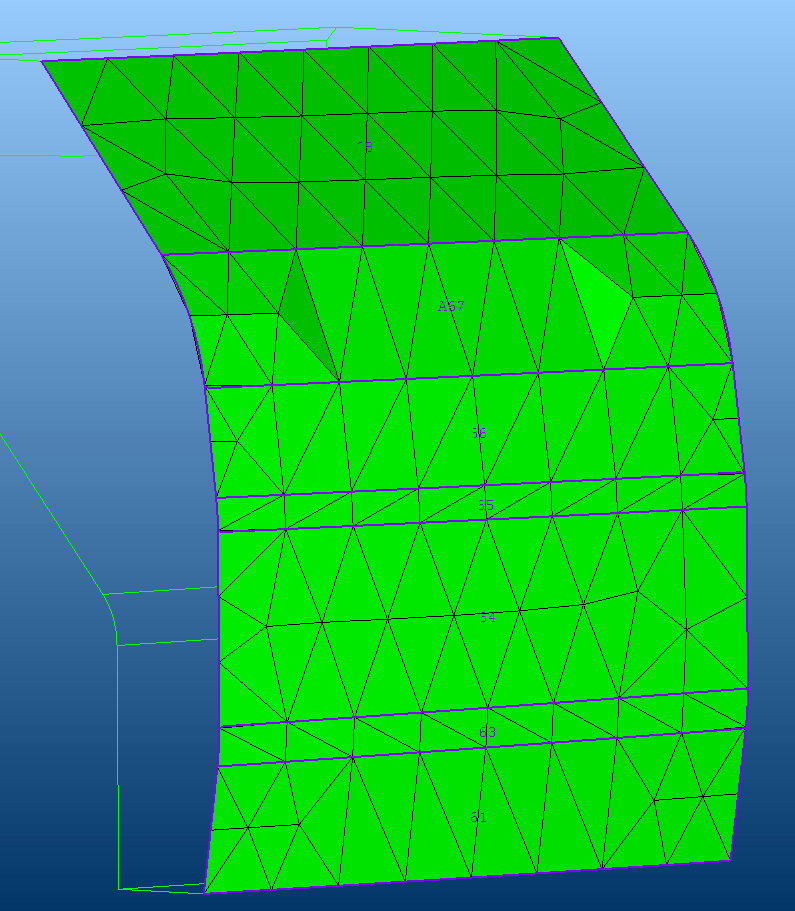
\includegraphics[width=0.4\columnwidth]{../png/t2t2}
}
\caption{
Different T1 meshes produced with (left) and without sag control (right).
The left plot has mesh features illustrates the gap between boundaing NURBS curve and NURBS surface,
caused in this case by defeaturing of fillets around the surface edges.
\label{fig:meshsag}}
\end{figure}

%32

\begin{figure}
\centerline{
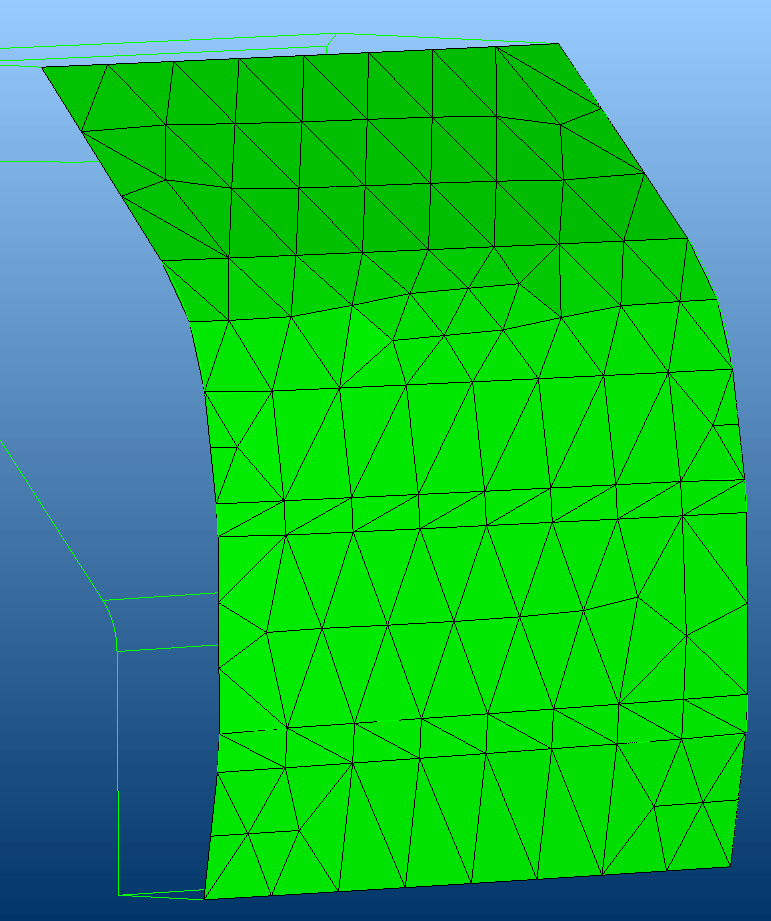
\includegraphics[width=0.33\columnwidth]{../png/t2t1}
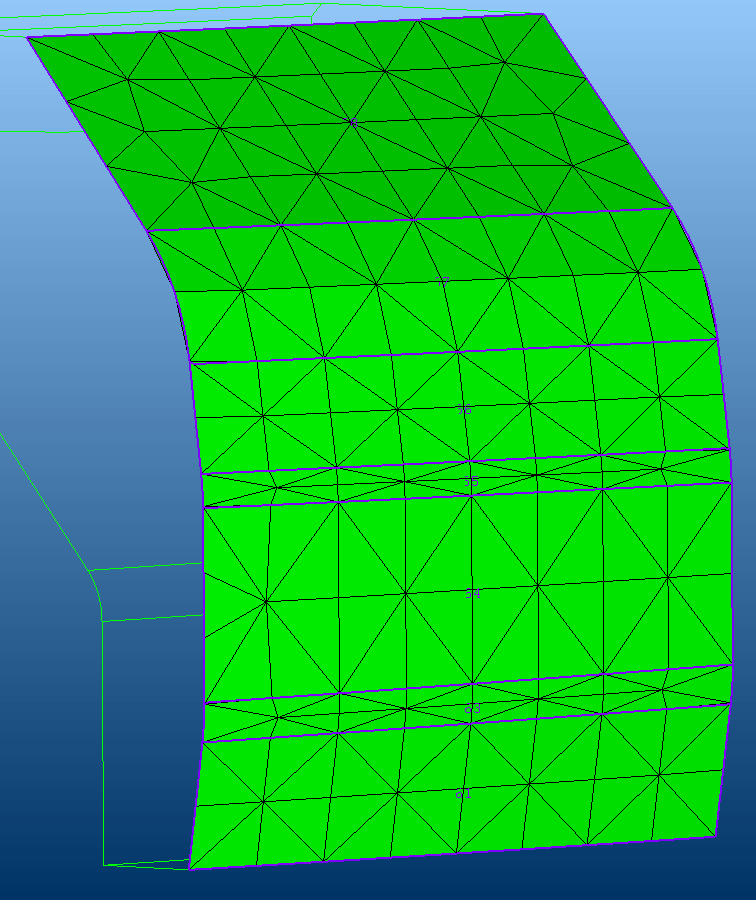
\includegraphics[width=0.33\columnwidth]{../png/t2t3}
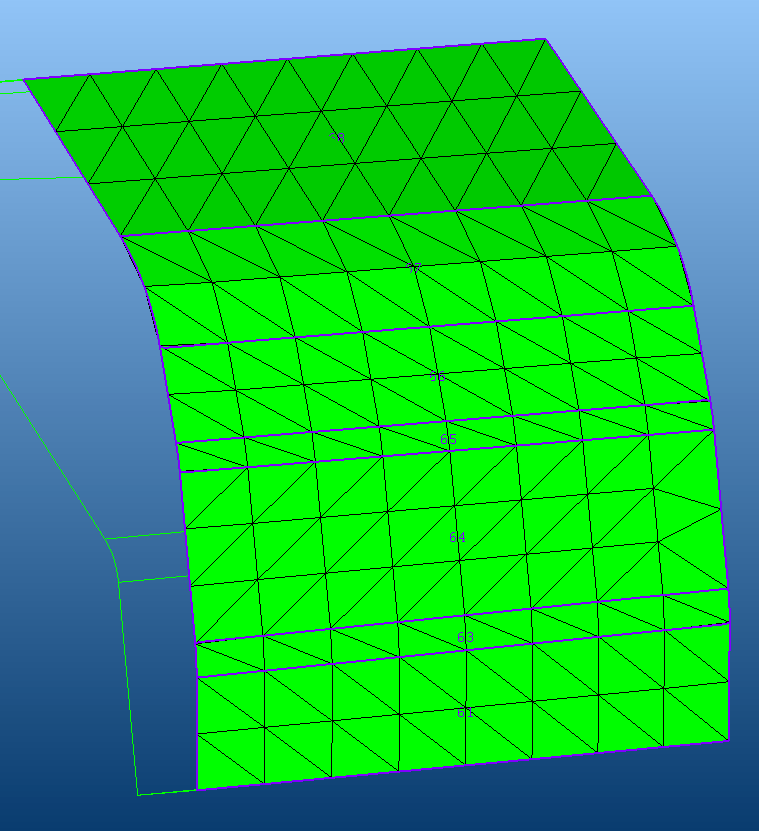
\includegraphics[width=0.35\columnwidth]{../png/t2t4}
}
\caption{
Exploration of the effect of different meshing controls on T1.
\label{fig:meshopt}}
\end{figure}

\begin{figure}
\centerline{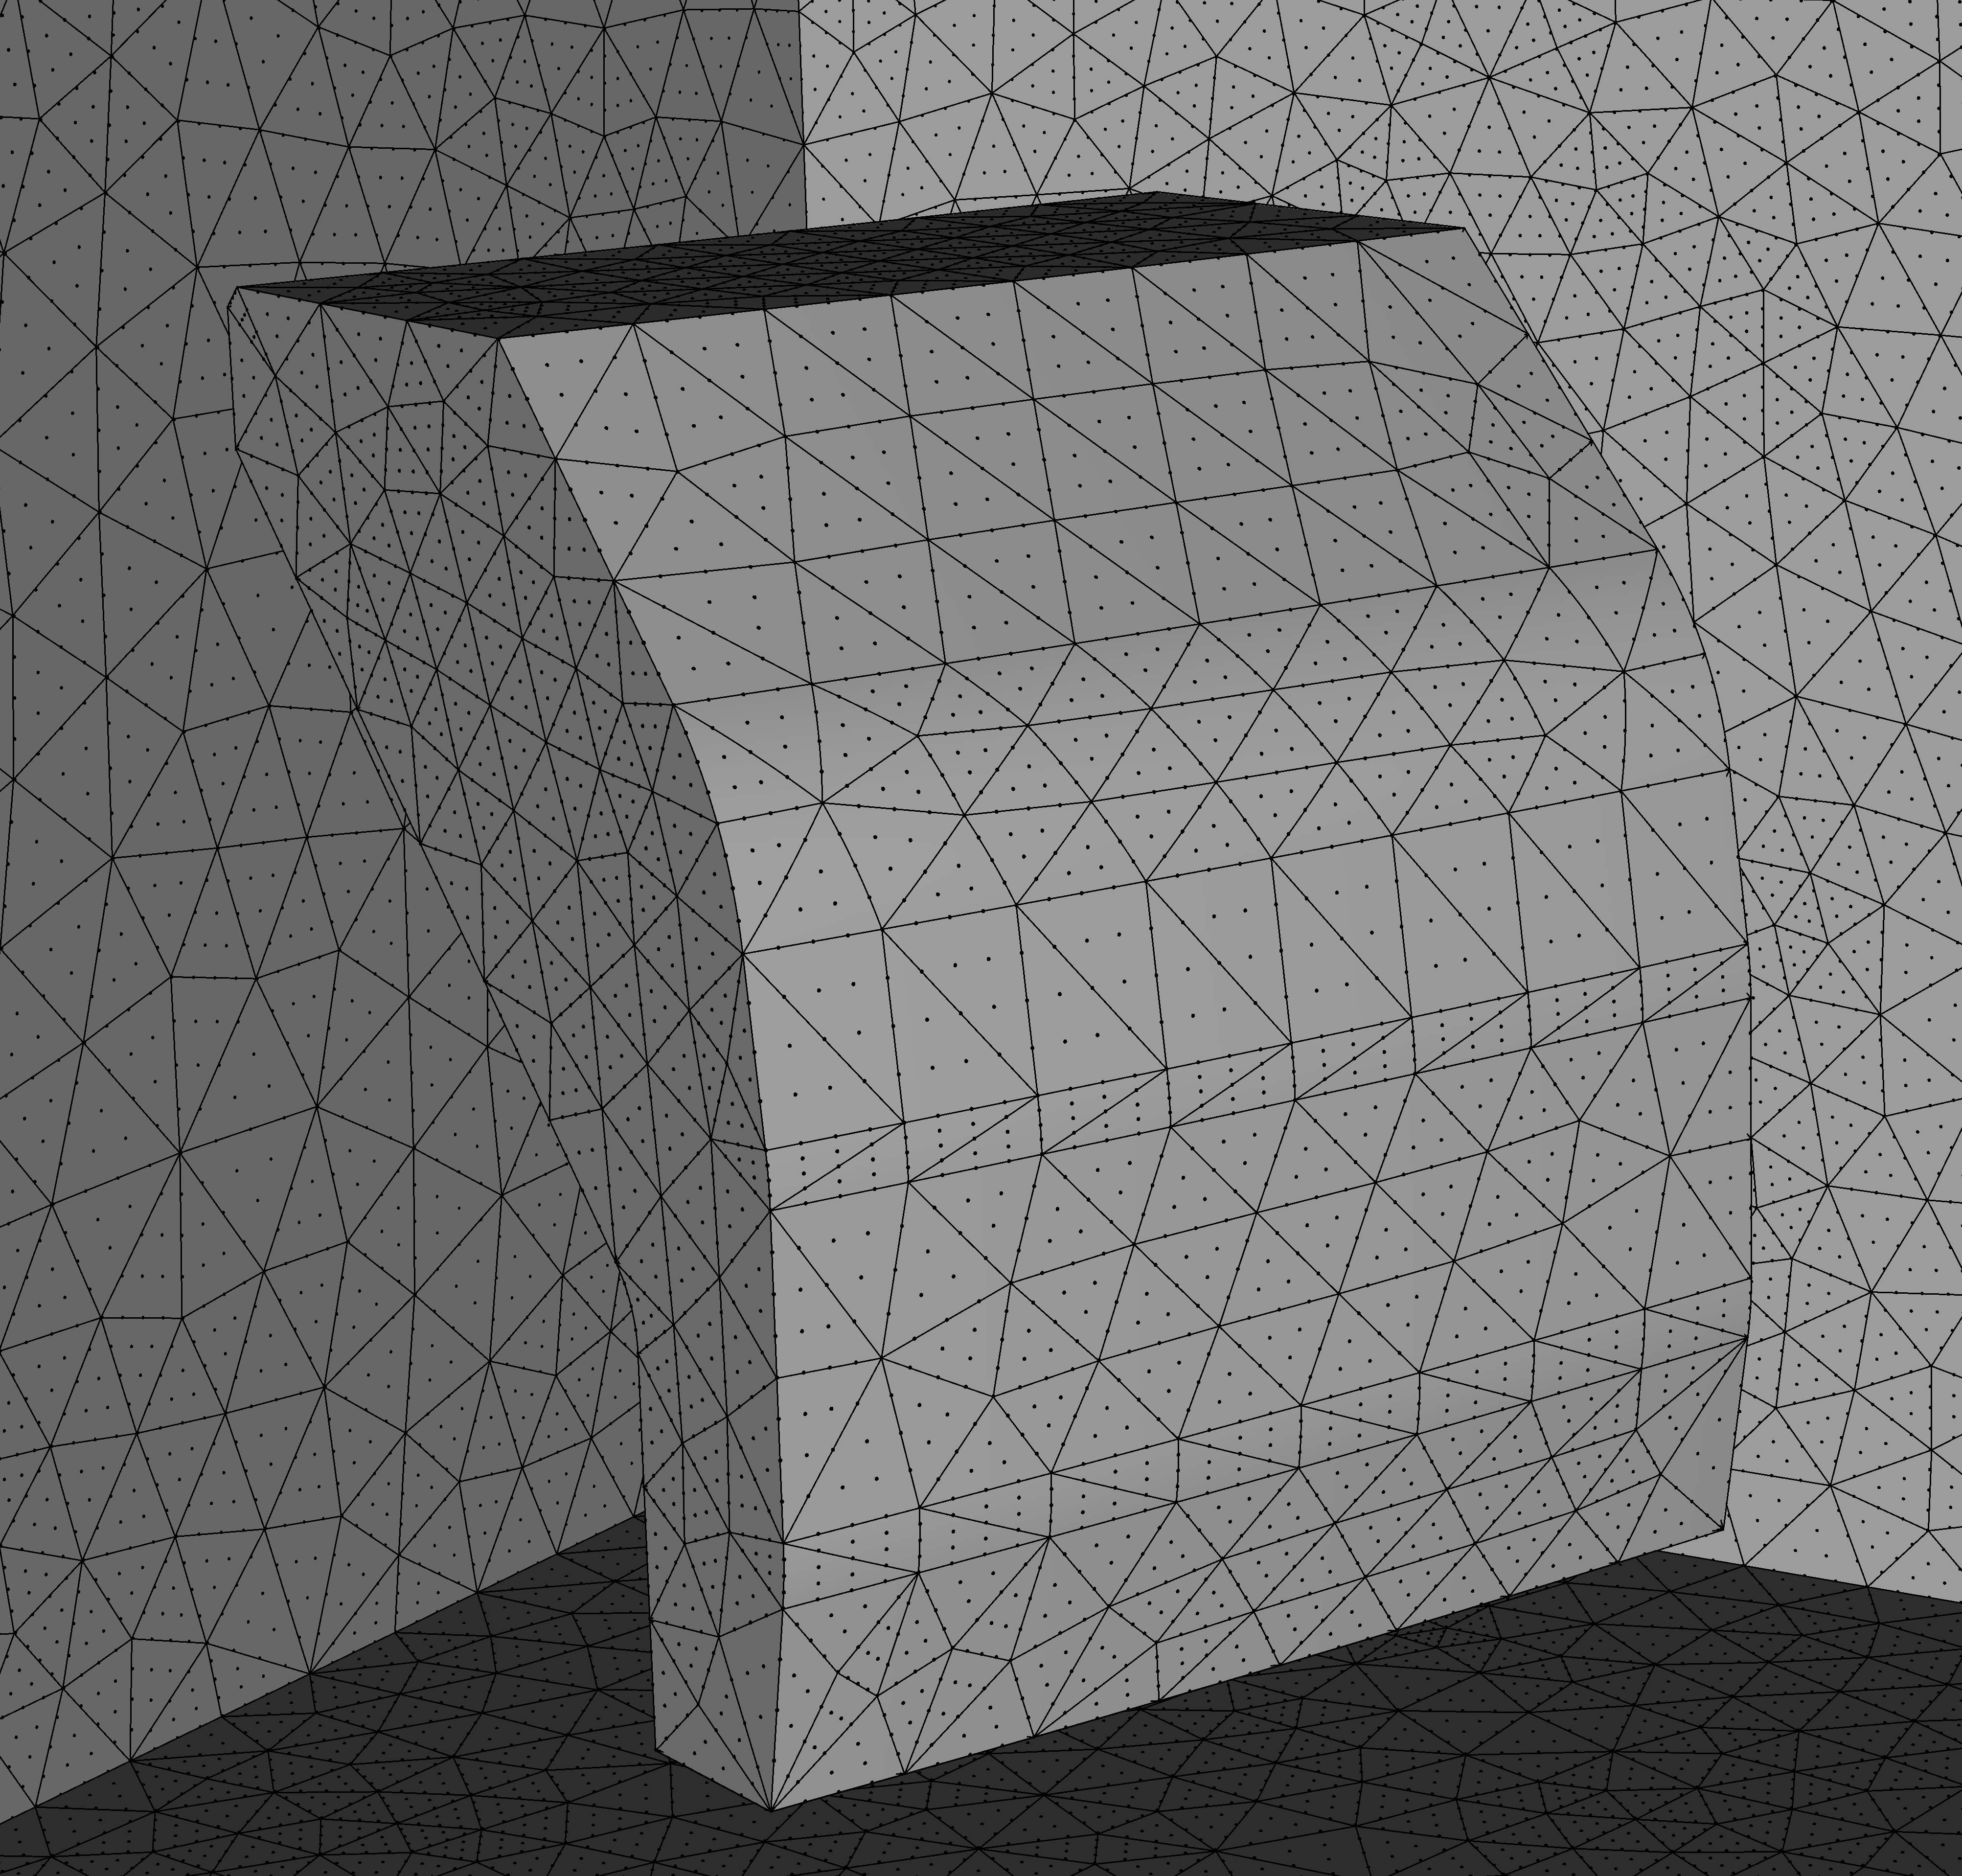
\includegraphics[width=8cm]{../png/visit0000}}
\caption{Meshing of JET T1 tile by D.~Moxey 6/3/20 using Nekmesh. The dots indicate nodes within
the non-planar triangular elements.\label{fig:visit0}}
\end{figure}


A sample text case is illustrated in \Fig{visit0} for the JET Tile~1,
which is one of the vertical tiles at the left of the divertor in \Fig{jetdive}.

\clearpage
\subsection{Element Shape Problem} \label{sec:eltprob}
\begin{figure}
\centerline{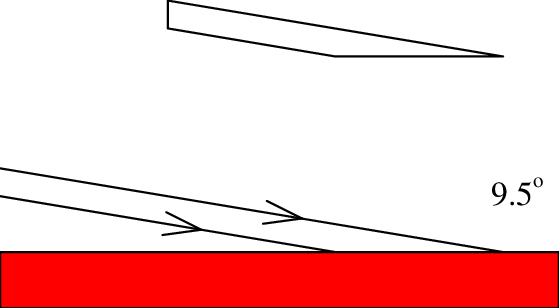
\includegraphics[width=8cm]{../png/9p5deg}}
\caption{Undesirable element shape if meshing conforms to both surface and fieldline.\label{fig:9p5deg}}
\end{figure}

Even assuming accurate meshing, there is a problem caused by the need to spread power
as widely as possible over the surfaces. Power is observed to flow along field lines, being
deposited proportionately as $\hat{\bf n}\cdot(\hat{\bf B}$, where  $\hat{\bf n}$ is
the unit normal to the surface and $(\hat{\bf B}$ gives
the direction of magnetic field~${\bf B}$.
Many designs call for a $2^o$~angle of field incidence on the surface. Such a small angle
is impossible to draw, the best that
is easily drawn is $9.5^o$ ($\arctan 1/6$), see \Fig{9p5deg} Elements with $2^o$ corners present such serious
challenges that simultaneous alignment with both the fieldlines and the geometry appears
to be a non-starter. The Science Plan~\cite{sciplan} recognises that it will be important to establish just
how large an anisotropy in the transport can be treated accurately without special coding.

%Fluid model of the edge : challenges
%1. Flow into engineered tile surface at
%approx. sonic speed following field
%Two-degree incidence design cf. 9.5o
%2. Magnetic field causes anisotropy
%3. Interaction with neutrals leads to large sources and sinks of mass and momentum
%4. Neutral particles are not necessarily Maxwellian distributed
%5. Plasma ion species often not accurately represented as fluid either
%6. Fluids may be 5-D or 6-D phase-fluids as well as 1-D to 3-D

